\documentclass[11pt,a4paper]{article}

\usepackage[utf8]{inputenc}
\usepackage[T1]{fontenc}
\usepackage{lmodern}
\usepackage{geometry}
\usepackage{graphicx}
\usepackage{booktabs}
\usepackage{amsmath}
\usepackage{amssymb}
\usepackage{hyperref}
\usepackage{xcolor}
\usepackage{enumitem}
\usepackage{caption}
\usepackage{subcaption}

\geometry{margin=1in}
\hypersetup{
    colorlinks=true,
    linkcolor=blue,
    citecolor=blue,
    urlcolor=blue
}

\title{Preliminary Data-Centric Study of Pulmonary Electrical Impedance Tomography with Atlas-Aware Continuous Conductivity Reconstruction}
\author{Anonymous Authors}
\date{}

\begin{document}
\maketitle

\begin{abstract}
Pulmonary electrical impedance tomography (EIT) differs from benchmark phantom reconstruction because the underlying conductivity fields are dominated by stable thoracic anatomy and only a relatively small portion of the image varies across samples. This paper presents a preliminary pulmonary EIT study based on synthetic thorax data generated within the KTC2023 codebase. We compare FCUNet-style image-space reconstruction, direct low-frequency DCT prediction, and several atlas-aware conductivity regressors. The experiments show that pulmonary conductivity prediction is strongly atlas-dominated: on a 2048-sample synthetic test split, a train-mean atlas baseline already achieves a masked relative-$L_2$ error of 0.2552, while a direct continuous DCT regressor degrades to 0.3509. Atlas-aware residual, hybrid, and atlas-decoder models recover the correct data regime but remain effectively tied to the atlas baseline globally and inside residual regions. In parallel, pulmonary segmentation on the same synthetic setting shows that FCUNet currently outperforms the DCT route in accuracy, whereas DCT remains substantially more efficient in parameter count and inference latency. Finally, a first matched 16-electrode time-difference study shows that local change structure can be recovered better than a zero predictor in active regions, but false positives still prevent global RMSE gains. These findings suggest that the key pulmonary bottleneck is no longer global image representation but measurement-to-residual inference. They also indicate that future pulmonary work should move toward 16-electrode matched simulation, residual or time-difference targets, and local deviation modeling rather than pure absolute-conductivity prediction.
\end{abstract}

\noindent\textbf{Keywords:} pulmonary EIT, conductivity regression, atlas prior, low-frequency reconstruction, residual imaging

\section{Introduction}
Pulmonary EIT is attractive for bedside monitoring because it is radiation-free, portable, and capable of measuring regional impedance changes in real time \cite{frerichs2017consensus}. At the same time, it is more structurally constrained than generic phantom reconstruction: the global thoracic outline is stable, whereas clinically meaningful change is often concentrated in relatively small local deviations such as regional ventilation loss, collapse, or fluid-related contrast.

This makes pulmonary EIT a poor fit for a naive interpretation of image reconstruction as unconstrained pixel prediction. A method that appears strong on benchmark phantoms may still fail on pulmonary data if it cannot separate stable global anatomy from measurement-driven local perturbations. The goal of this preliminary paper is therefore not to claim a final pulmonary solution, but to document what the current repository already reveals about pulmonary representation bias.

At the same time, the exploratory branch should not remain closed within only custom architectures. Pulmonary EIT already has a widely used classical reconstruction route, namely GREIT \cite{adler2009greit}, and it also has reusable Python tooling through pyEIT \cite{liu2018pyeit}. Recent pulmonary deep-learning work such as Zeng et al. \cite{zeng2023lungdl} further suggests that lung tdEIT benefits from representation-aware learning under matched measurement protocols. For that reason, the current pulmonary study is now being repositioned as a two-stage process: first reproduce externally grounded pulmonary baselines, and then adapt the repository's own DCT / residual ideas on top of them.

\section{Study Setting}
\subsection{Synthetic Pulmonary Data}
The repository currently contains synthetic thorax-style datasets with two lungs, a heart-like region, and configurable local pathology perturbations. The main datasets used in this paper are:
\begin{itemize}[leftmargin=1.5em]
    \item \texttt{dataset\_lung\_2k}: 2048 samples in the current 32-electrode, 2356-channel KTC-style measurement format;
    \item \texttt{dataset\_lung\_varlow}: 512 samples with weaker anatomical and local perturbation complexity;
    \item \texttt{dataset\_lung\_varhigh}: 512 samples with stronger anatomy variation, pathology variation, and conductivity texture.
\end{itemize}

These data support both a segmentation-style evaluation and a continuous conductivity-regression evaluation.

\subsection{Real Thoracic Measurements}
The repository also includes real thoracic \texttt{.get} files from a PLOS One dataset related to lung-heart separation in EIT \cite{li2021thorax}. We verified that these recordings follow a 16-electrode acquisition layout and reduce to 208 valid channels after DCT-EIT-style reordering. This is important because it means the current 32-electrode neural pipelines are not yet directly matched to the real pulmonary measurement regime.

\subsection{Methods}
The main pulmonary methods examined so far are:
\begin{itemize}[leftmargin=1.5em]
    \item FCUNet segmentation baseline;
    \item DCT predictor for pulmonary segmentation;
    \item direct DCT conductivity regression;
    \item atlas-residual DCT conductivity regression;
    \item hybrid atlas + coarse DCT + local refinement regression;
    \item atlas-decoder regression with a learned atlas-aware residual decoder;
    \item FC-SigmaUNet as a heavier continuous image-space baseline.
\end{itemize}

\section{Pulmonary Segmentation Results}
On the current 2048-sample synthetic pulmonary segmentation task, FCUNet remains the stronger baseline:
\begin{itemize}[leftmargin=1.5em]
    \item FCUNet mean score: 0.7819,
    \item DCT predictor mean score: 0.7272,
    \item DCT predictor ensemble mean score: 0.7269.
\end{itemize}

However, the DCT route remains much more efficient:
\begin{itemize}[leftmargin=1.5em]
    \item DCT predictor: 3.85M parameters, 2.14 ms single-sample latency, 0.25 ms/sample at batch=32;
    \item FCUNet: 40.70M parameters, 28.82 ms single-sample latency, 14.60 ms/sample at batch=32.
\end{itemize}

\begin{figure}[htbp]
    \centering
    \begin{subfigure}{0.48\linewidth}
        \centering
        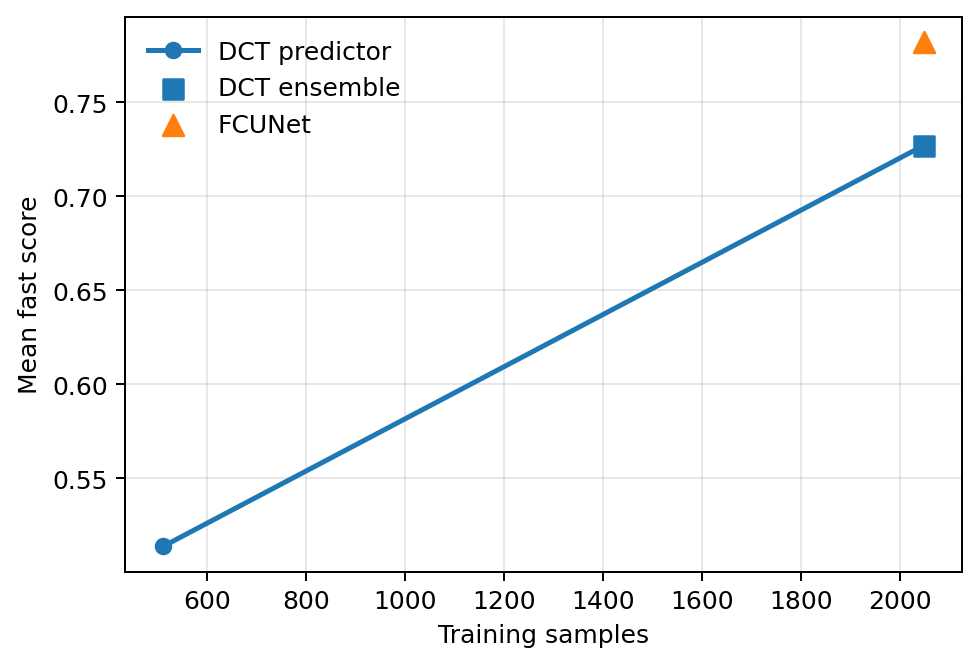
\includegraphics[width=\linewidth]{../../results/pulmonary_summary_1/pulmonary_score_scaling.png}
    \end{subfigure}
    \hfill
    \begin{subfigure}{0.48\linewidth}
        \centering
        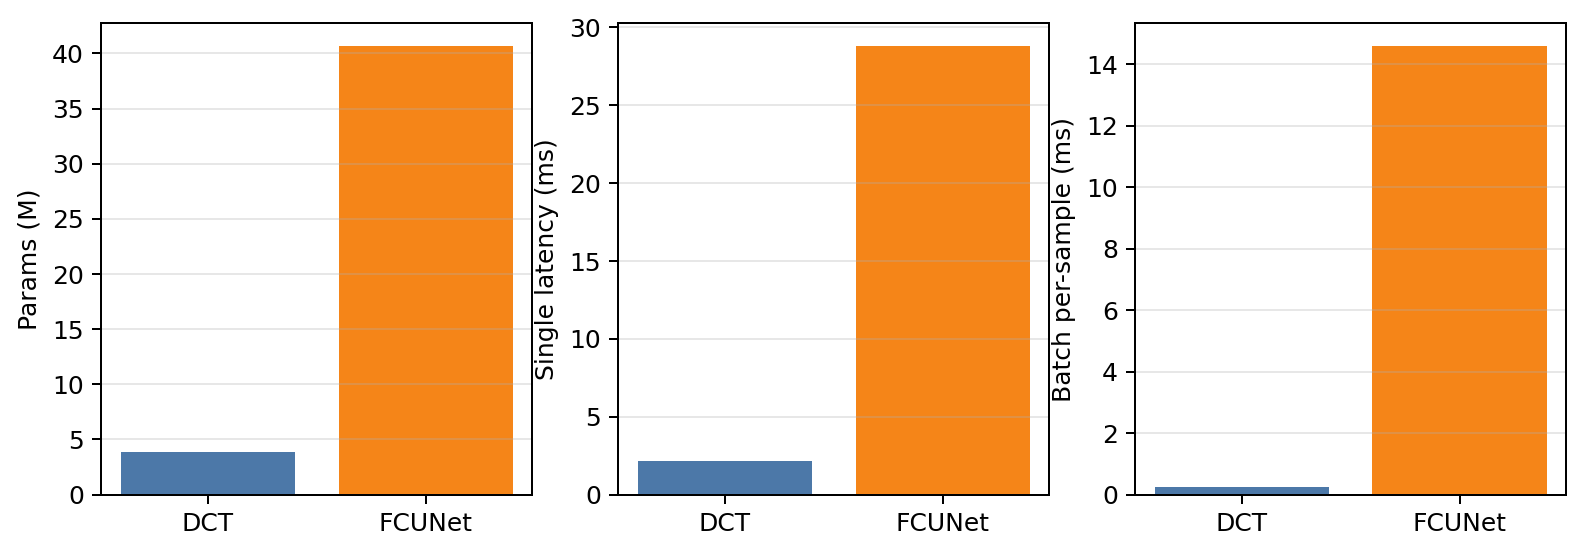
\includegraphics[width=\linewidth]{../../results/pulmonary_summary_1/pulmonary_efficiency.png}
    \end{subfigure}
    \caption{Pulmonary segmentation summary. Left: DCT data-scaling behavior. Right: DCT versus FCUNet efficiency comparison.}
    \label{fig:pulmonary-summary}
\end{figure}

Therefore, the pulmonary segmentation evidence currently supports an efficiency-oriented role for DCT rather than a best-accuracy claim.

\section{Continuous Conductivity Regression}
\subsection{Atlas Dominance}
The most important conductivity-regression result is that pulmonary synthetic data are strongly atlas-dominated. On \texttt{dataset\_lung\_2k}, a trivial train-mean atlas baseline already achieves:
\[
\mathrm{RelL2} \approx 0.2552.
\]

By contrast, the first direct continuous DCT regressor degrades to:
\[
\mathrm{RelL2} \approx 0.3509.
\]

So the pulmonary problem is not primarily ``recover the whole thorax from scratch'', but rather ``recover small local deviations around a stable anatomical template''.

\subsection{Atlas-Aware Adaptation}
To match this structure, we implemented three atlas-aware models:
\begin{itemize}[leftmargin=1.5em]
    \item atlas-residual DCT,
    \item hybrid DCT with coarse and local branches,
    \item atlas-decoder with a learned residual image decoder.
\end{itemize}

On \texttt{dataset\_lung\_2k}, all three return almost exactly to the atlas baseline:
\begin{itemize}[leftmargin=1.5em]
    \item atlas-residual DCT: 0.2552,
    \item hybrid DCT: 0.2552,
    \item atlas-decoder: 0.2552.
\end{itemize}

This means atlas-aware adaptation prevents collapse, but does not yet yield a meaningful improvement beyond the atlas itself.

\subsection{Complexity-Matched Evidence}
The same conclusion also holds on matched low/high-complexity pulmonary datasets. In low complexity:
\begin{itemize}[leftmargin=1.5em]
    \item atlas baseline: 0.1990,
    \item direct DCT: 0.6944,
    \item atlas-residual DCT: 0.2008,
    \item hybrid DCT: 0.2012,
    \item atlas-decoder: 0.2006,
    \item FC-SigmaUNet pilot: 0.2049.
\end{itemize}

In high complexity:
\begin{itemize}[leftmargin=1.5em]
    \item atlas baseline: 0.2995,
    \item direct DCT: 0.7230,
    \item atlas-residual DCT: 0.2971,
    \item hybrid DCT: 0.2973,
    \item atlas-decoder: 0.2972,
    \item FC-SigmaUNet pilot: 0.3010.
\end{itemize}

\begin{figure}[htbp]
    \centering
    \begin{subfigure}{0.48\linewidth}
        \centering
        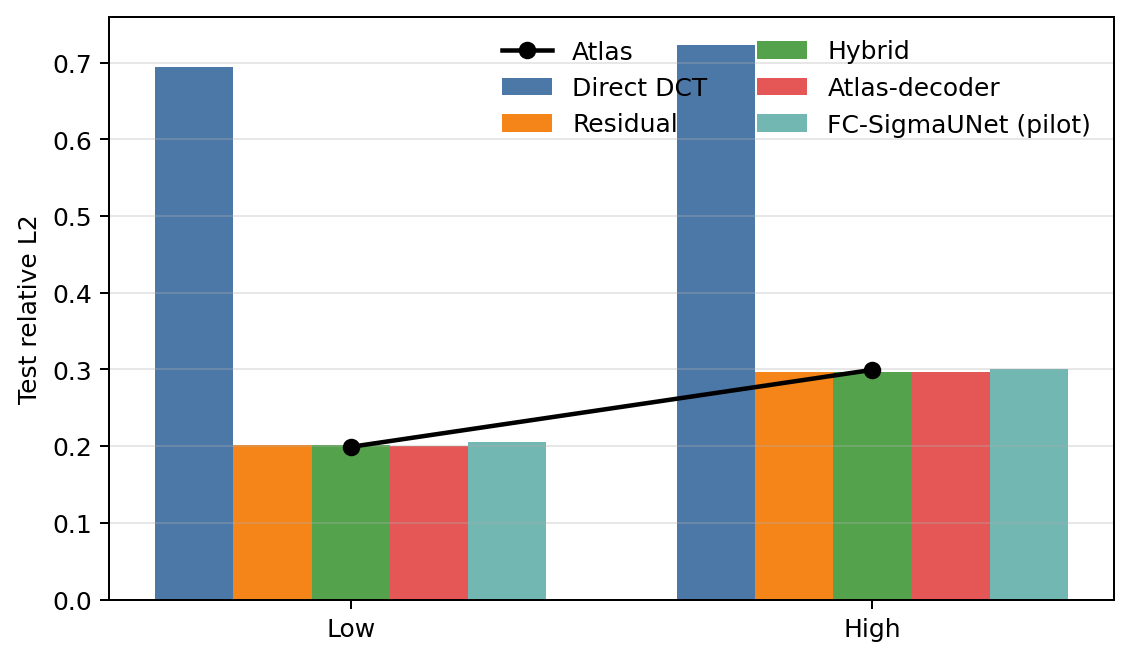
\includegraphics[width=\linewidth]{../../results/pulmonary_complexity_models_3/complexity_bar.png}
    \end{subfigure}
    \hfill
    \begin{subfigure}{0.48\linewidth}
        \centering
        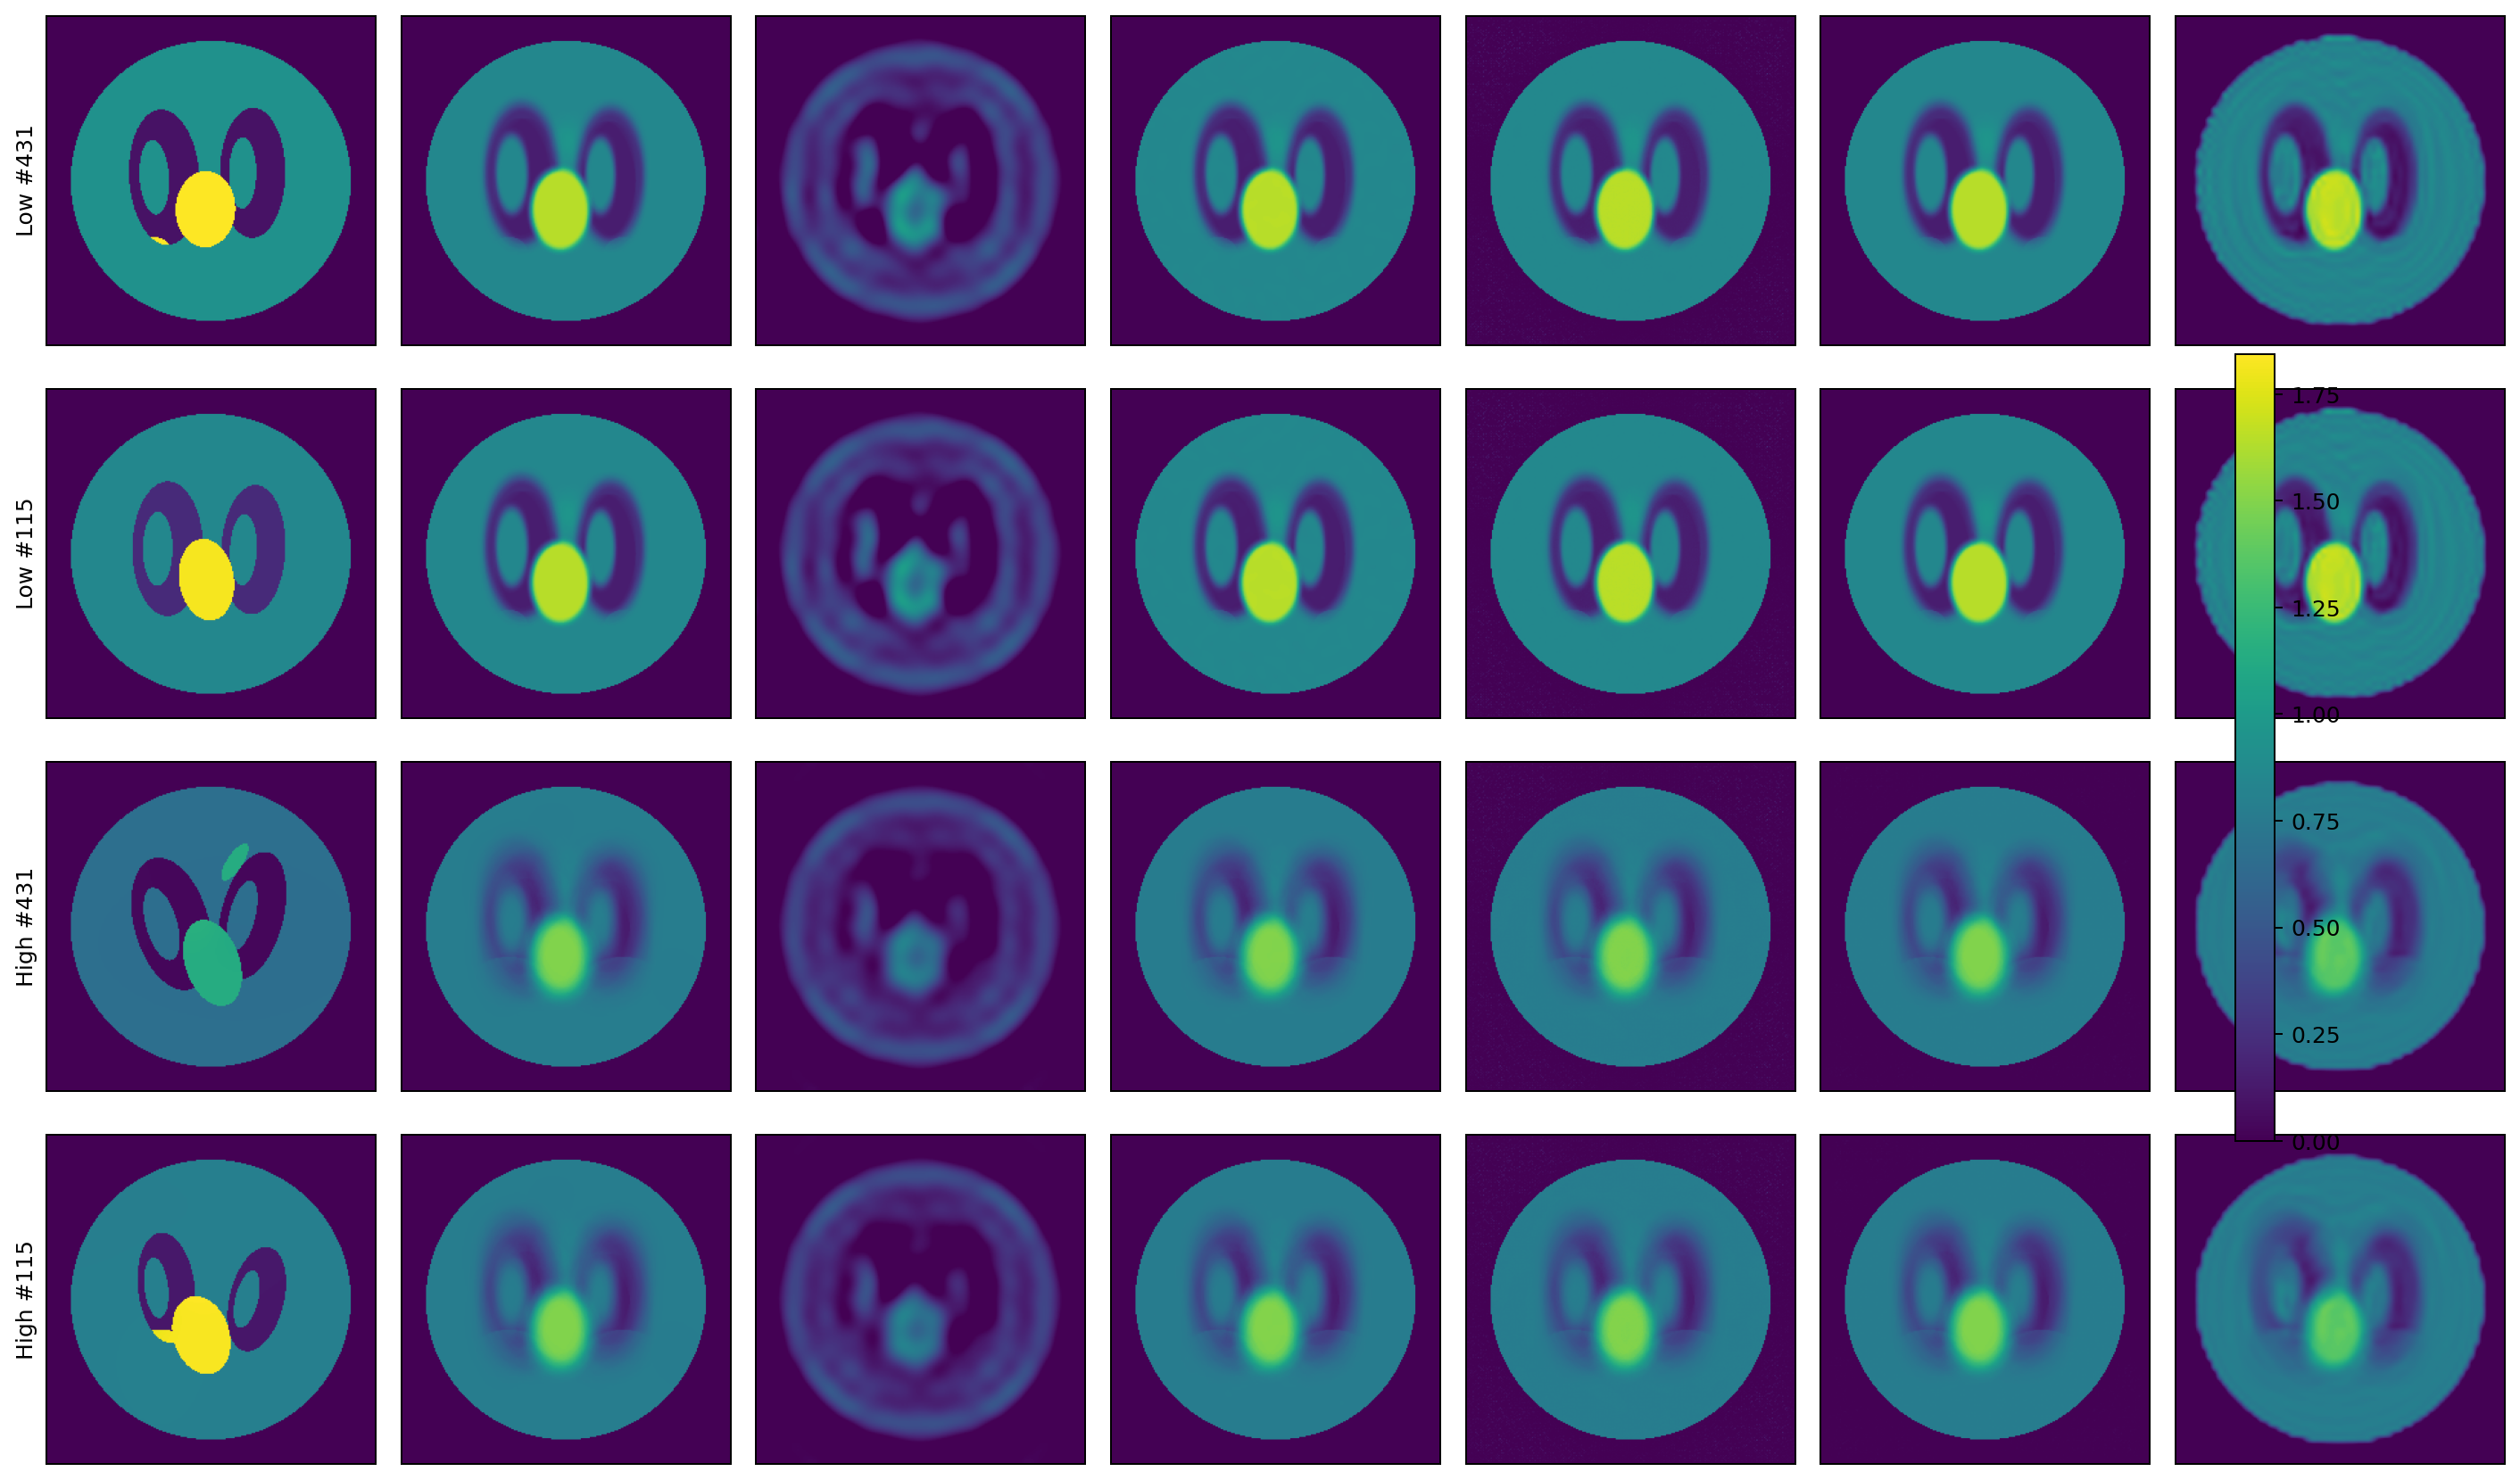
\includegraphics[width=\linewidth]{../../results/pulmonary_complexity_visual_3/comparison.png}
    \end{subfigure}
    \caption{Matched low/high-complexity pulmonary conductivity results. Left: relative-$L_2$ summary. Right: qualitative comparison.}
    \label{fig:complexity}
\end{figure}

These experiments indicate that the core pulmonary challenge is not decoder capacity. Even a much heavier FC-SigmaUNet pilot stays near the same atlas-dominated operating point.

\section{Residual-Focused Analysis}
Global relative-$L_2$ can still hide whether a model actually improves inside the deviation regions that matter clinically. We therefore evaluated only pixels satisfying
\[
|\sigma - \sigma_{\text{atlas}}| > 0.08.
\]

On \texttt{dataset\_lung\_2k}, the residual-region relative-$L_2$ values are:
\begin{itemize}[leftmargin=1.5em]
    \item atlas: 0.3746,
    \item atlas-residual DCT: 0.3747,
    \item hybrid DCT: 0.3747,
    \item atlas-decoder: 0.3746.
\end{itemize}

So the atlas-aware models do not merely \emph{appear} tied to the atlas globally; they are also essentially tied to the atlas in the local deviation regions themselves.

\begin{figure}[htbp]
    \centering
    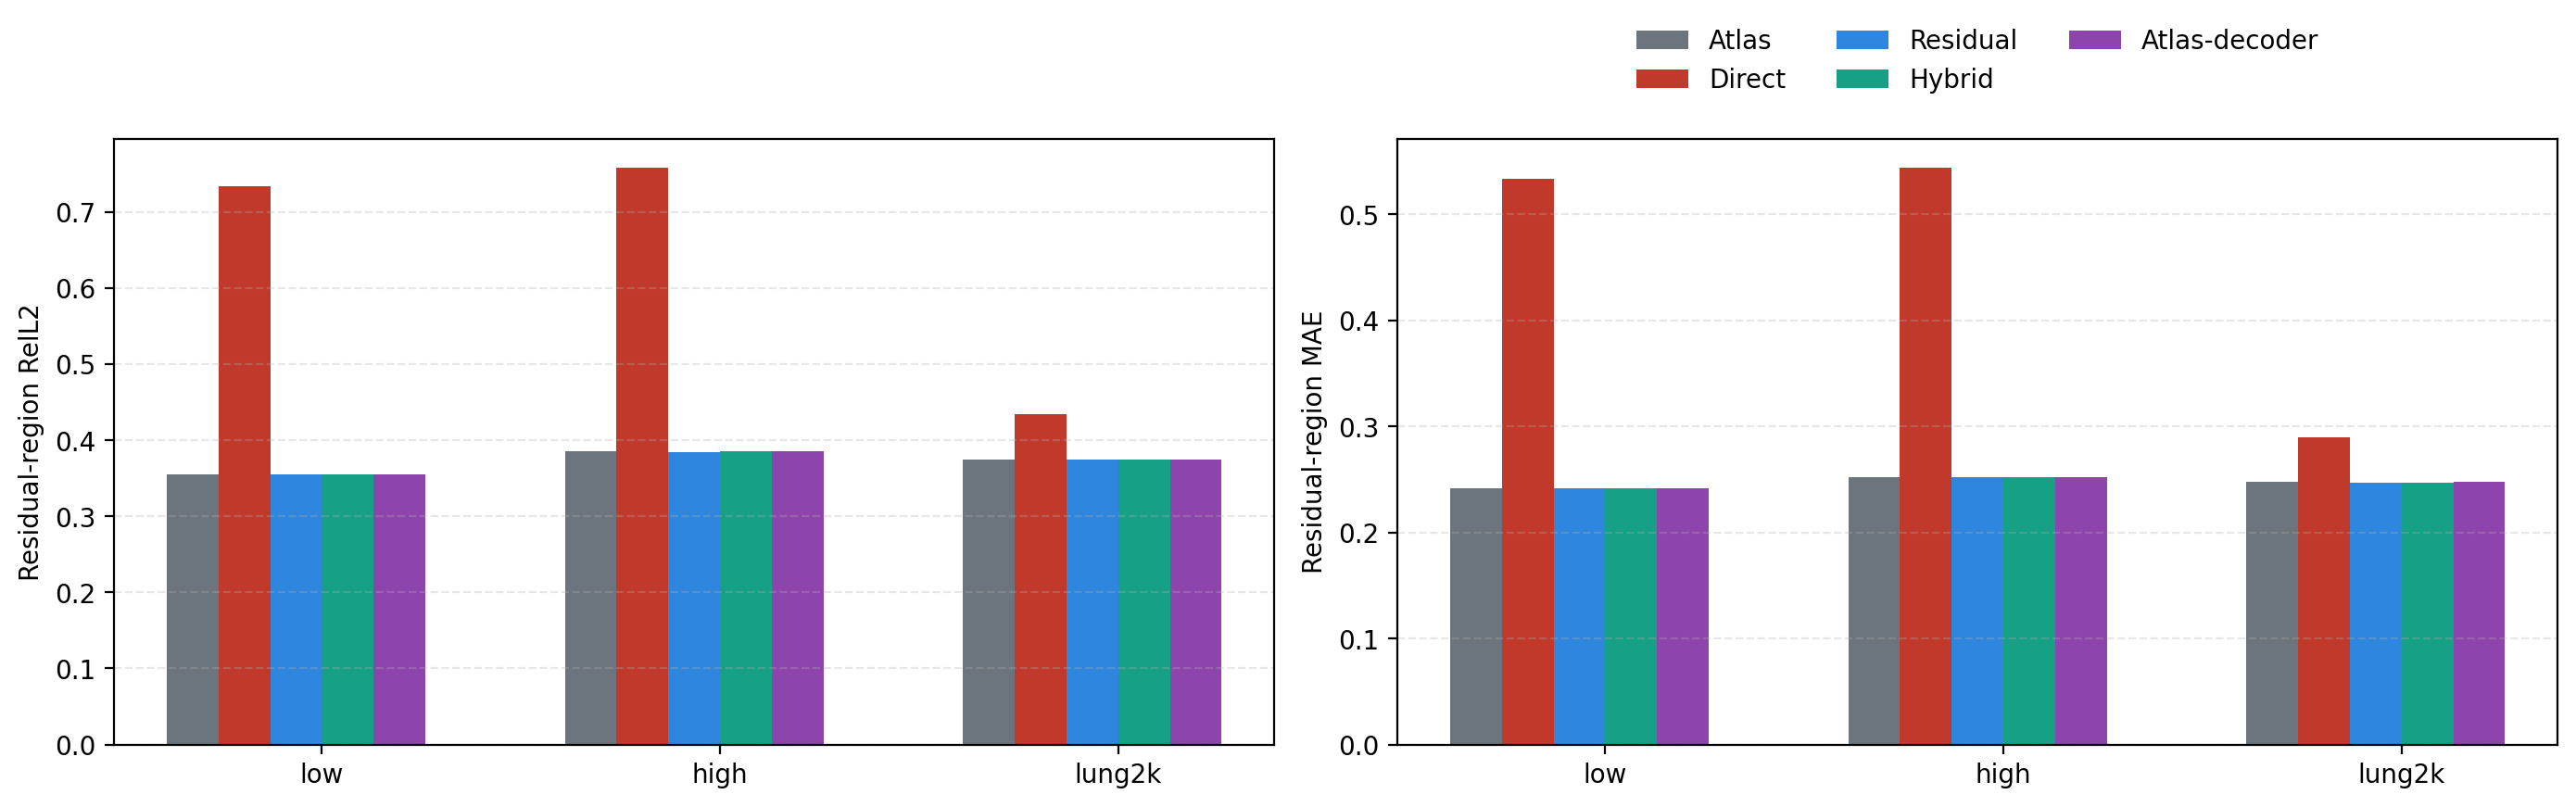
\includegraphics[width=0.74\linewidth]{../../results/pulmonary_residual_focus_2/residual_focus_bar.png}
\caption{Residual-focused pulmonary analysis using deviation-region metrics.}
\label{fig:residual-focus}
\end{figure}

We also checked whether a focus-weighted residual loss was the missing ingredient. It was not. Removing focus weighting changes low-complexity relative-$L_2$ from 0.2008 to 0.2007 and high-complexity relative-$L_2$ from 0.2971 to 0.2972. Hence simple loss reweighting is not the real bottleneck.

\section{Matched 16-Electrode Time-Difference Exploration}
The real thoracic recordings in this repository are not only pulmonary in
content; they are also acquired under a different measurement regime from the
32-electrode KTC-style synthetic chain. To reduce that mismatch, I implemented a
first matched 16-electrode simulation and learning pipeline:
\begin{itemize}[leftmargin=1.5em]
    \item paired pulmonary phantoms with a reference state and a target state,
    \item raw 256-channel measurement simulation,
    \item DCT-EIT-style $256 \rightarrow 208$ channel reordering,
    \item direct prediction of continuous conductivity change $\Delta \sigma$
    from reordered delta measurements.
\end{itemize}

This new line should be interpreted as an exploratory bridge toward realistic
pulmonary EIT rather than a final model.

\subsection{Classical GREIT Reproduction}
To avoid evaluating the TD16 branch only against internal neural baselines, I
also reproduced a classical GREIT baseline using pyEIT \cite{liu2018pyeit} and
a custom \texttt{Draeger 208} protocol aligned to the local
\texttt{256 -> 208} channel reordering. This is important because GREIT is
still the most standard pulmonary linear reconstruction family in practice
\cite{adler2009greit}, and because the real thoracic \texttt{.get} data in this
repository follow the same \texttt{16}-electrode measurement regime.

On the mixed TD16 pilot, the reproduced GREIT baseline reaches:
\begin{itemize}[leftmargin=1.5em]
    \item thorax mesh: RMSE$_{32} = 0.0859$, active-region relative-$L_2 = 1.0034$,
    \item circle mesh: RMSE$_{32} = 0.0851$, active-region relative-$L_2 = 0.9951$.
\end{itemize}

On the active-only TD16 pilot:
\begin{itemize}[leftmargin=1.5em]
    \item thorax mesh: RMSE$_{32} = 0.1205$, active-region relative-$L_2 = 0.9910$,
    \item circle mesh: RMSE$_{32} = 0.1279$, active-region relative-$L_2 = 1.0203$.
\end{itemize}

These numbers are not yet strong pulmonary results, but they matter for two
reasons. First, they show that a classical pulmonary baseline can now be
reproduced under the same local TD16 measurement protocol rather than only
discussed abstractly. Second, they indicate that the current learned TD16
models are already competing with, and in some settings surpassing, a matched
GREIT baseline even though they still do not outperform the zero predictor
globally on mixed data.

\subsection{Approximate VAE-Manifold Reproduction}
To move beyond classical baselines, I also implemented an approximate
reproduction of the manifold-learning route described by Zeng et al.
\cite{zeng2023lungdl}. The local approximation keeps the same high-level idea:
first train a variational autoencoder on TD16 conductivity-change images, then
train a multilayer perceptron to map TD16 measurements into the learned latent
space, and finally decode the latent prediction back to conductivity-change
images. The exact CT-derived 15000-pair training pipeline of the original paper
is not yet available locally, so the present implementation should be treated
as a matched-protocol approximation rather than a faithful end-to-end
reproduction.

On the active-only TD16 pilot, the VAE autoencoder itself achieves RMSE
$= 0.1189$ and active-region relative-$L_2 = 0.7587$, while the latent
predictor degrades to RMSE $= 0.1315$ and active-region relative-$L_2 = 0.9692$.
This indicates that, under active-only conditions, the dominant bottleneck is
the inverse mapping from measurements to latent variables rather than the image
manifold. On the mixed TD16 pilot, however, the story changes: the VAE
autoencoder already collapses near the weak-change operating point
(RMSE $= 0.0856$, active-region relative-$L_2 = 0.9983$), and the latent
predictor remains essentially tied to that weak manifold
(RMSE $= 0.0842$, active-region relative-$L_2 = 0.9983$). Therefore, the
manifold-learning route is plausible only when the data regime is already
change-dominant; once zero-change samples dominate, the learned manifold itself
becomes too insensitive to sparse local changes.

I further tested a two-stage combination in which a mixed-data external
mask-only localizer gates the output of an active-only VAE predictor. This
reduces the mixed-pilot RMSE from $0.0891$ to $0.0862$, but the active-region
relative-$L_2$ worsens from $0.9525$ to $0.9753$. So stronger localization can
indeed suppress false positives for the VAE route, yet it still does not solve
the actual amplitude recovery problem in the active region.

I then made the coupling tighter by training a mask-conditioned latent
predictor in which the mixed-data predictor explicitly regresses a low-frequency
spatial mask and feeds that mask representation into the latent head. This
reduces the mixed-pilot active-region relative-$L_2$ to $0.9686$, but the
global RMSE remains $0.0886$, which is still worse than both the mixed VAE
predictor ($0.0842$) and the simpler external soft-fusion strategy ($0.0862$).
Therefore, the failure is not simply that the latent predictor never sees
localization cues. The remaining problem is that localization and residual
amplitude recovery are still not coupled in a sufficiently effective way.

\subsection{Mixed Pilot with Zero-Change Cases}
On a 64-sample pilot dataset containing both active-change and near-zero-change
pairs, the zero predictor remains a strong global baseline:
\begin{itemize}[leftmargin=1.5em]
    \item zero baseline: RMSE $= 0.0835$, active-region relative-$L_2 = 1.0000$,
    \item TD16 predictor: RMSE $= 0.0958$, active-region relative-$L_2 = 0.9788$.
\end{itemize}

The zero-delta fraction is $42.9\%$. This means the learned model begins to
recover some local change structure better than the trivial baseline, but false
positives still hurt the global RMSE.

\subsection{Active-Only Pilot}
When the zero-change proportion is reduced, the same pattern becomes clearer:
\begin{itemize}[leftmargin=1.5em]
    \item zero baseline: RMSE $= 0.1314$, active-region relative-$L_2 = 1.0000$,
    \item TD16 predictor: RMSE $= 0.1321$, active-region relative-$L_2 = 0.9228$.
\end{itemize}

So once the task focuses on actual pulmonary change, the model starts to beat
the zero predictor in local change reconstruction, but it still does not
surpass it on global RMSE.

\subsection{Sparse TD16 Follow-Up}
To suppress diffuse false positives, I added inactive-region upweighting and a
weak prediction $L_1$ sparsity term. This improves local change recovery
further, but again at the cost of worse global RMSE:
\begin{itemize}[leftmargin=1.5em]
    \item mixed sparse TD16: RMSE $= 0.1038$, active-region relative-$L_2 = 0.9255$,
    \item active-only sparse TD16: RMSE $= 0.1353$, active-region relative-$L_2 = 0.9129$.
\end{itemize}

I then added a sample-level change-aware gate that predicts whether a meaningful
conductivity deviation exists and scales the residual output accordingly. On the
mixed pilot, this gate improves the trade-off relative to sparse-only TD16:
\begin{itemize}[leftmargin=1.5em]
    \item gate only: RMSE $= 0.1012$, active-region relative-$L_2 = 0.9521$,
    \item gate + sparse: RMSE $= 0.1007$, active-region relative-$L_2 = 0.9525$.
\end{itemize}

I then replaced the sample-level gate with a spatial change-mask branch. This
model predicts both low-frequency conductivity change and a low-frequency binary
change mask, and multiplies the two. On the mixed pilot, this becomes the best
learned TD16 variant so far:
\begin{itemize}[leftmargin=1.5em]
    \item spatial-mask TD16: RMSE $= 0.0923$, active-region relative-$L_2 = 0.9620$.
\end{itemize}

This is better than the original mixed TD16 (`0.0958`, `0.9788`) and better
than the sample-gated variants in global RMSE. On the active-only pilot, the
same spatial-mask design reaches:
\begin{itemize}[leftmargin=1.5em]
    \item RMSE $= 0.13136$,
    \item active-region relative-$L_2 = 0.9463$.
\end{itemize}

This almost exactly matches, and very slightly improves upon, the active-only
zero baseline RMSE (`0.13139`) while still outperforming the zero predictor in
active-region reconstruction. Therefore explicit spatial change localization is
currently the most promising pulmonary TD16 direction in this repository.

I also tested active-sample oversampling on the mixed pilot. It does not change
the conclusion: the oversampled spatial-mask model reaches RMSE $= 0.0925$ and
active-region relative-$L_2 = 0.9608$, which is effectively tied to the
non-oversampled spatial-mask model. So the remaining bottleneck is not merely
sample imbalance.

However, even the best mixed-data spatial-mask variant still does not beat the
mixed-data zero predictor on global RMSE (`0.0835`). Therefore the next
pulmonary step should not be a larger absolute-image decoder. It should be a
more explicit change-aware model that jointly addresses:
\begin{itemize}[leftmargin=1.5em]
    \item change/no-change detection,
    \item local residual reconstruction,
    \item false-positive suppression in near-zero regions.
\end{itemize}

I tested one such follow-up directly by conditioning the residual coefficient
branch on the predicted low-frequency spatial mask coefficients. This
conditional variant also supports mask teacher forcing during training. The
result is informative but not yet decisive. On the mixed pilot, conditional
residual regression reaches RMSE $= 0.0950$ and active-region
relative-$L_2 = 0.9504$, which is still worse than the simpler spatial-mask
model (`0.0923`, `0.9620`). Full teacher forcing does not improve the result.
On the active-only pilot, the conditional model slightly lowers global RMSE to
$0.13131$, marginally below the spatial-mask model (`0.13136`) and the zero
baseline (`0.13139`), but it still does not beat the original active-only TD16
model in local change recovery. Hence the remaining issue is no longer just
whether spatial change should be modeled explicitly; it is how to couple change
localization with residual amplitude estimation more effectively.

To sharpen that diagnosis, I added an oracle-mask analysis. The trained model is
kept fixed, but the predicted spatial mask is replaced at evaluation time by
the ground-truth change mask. For the conditional model, I also tested an even
stronger oracle in which the residual branch is conditioned on the ground-truth
low-frequency mask coefficients. This experiment reveals the current bottleneck
very clearly. On the mixed pilot, the spatial-mask TD16 model improves from
RMSE $= 0.0923$ to $0.0771$ under oracle masking, and the conditional model
improves further to $0.0739$ when both oracle conditioning and oracle masking
are provided. On the active-only pilot, the corresponding best oracle result is
RMSE $= 0.1137$, again far below the learned standard-output result
(`0.1313`). Therefore the residual branch is already capable of reconstructing
local pulmonary change better than the raw benchmark numbers imply. The
dominant remaining TD16 error now appears to be spatial change localization
rather than residual amplitude regression itself.

To test that diagnosis more directly, I then trained a dedicated mask-only TD16
predictor whose sole target is the binary spatial change region
$1(|\Delta \sigma| > 0.02)$. This dedicated mask head indeed outperforms the
internal mask branches learned jointly inside the residual models. On the mixed
pilot, the external mask predictor reaches mask IoU $= 0.0545$, compared with
$0.0285$ for the spatial TD16 internal mask and $0.0359$ for the conditional
TD16 internal mask. On the active-only pilot, the dedicated mask head improves
further to mask IoU $= 0.0898$, again above the internal spatial and conditional
mask branches (`0.0436` and `0.0535` respectively). This confirms that
localization quality can be improved by specializing the objective.

However, a second result is equally important: simply taking this better
external mask and multiplying it with the existing residual predictions does not
produce a strong global reconstruction gain. On the mixed pilot, external soft
fusion with the best spatial residual model yields RMSE $= 0.0926$, essentially
tied with the original spatial TD16 result (`0.0923`). On the active-only
pilot, the same external-mask fusion again produces an almost exact tie in
global RMSE. So the updated pulmonary TD16 conclusion is slightly more specific
than before. The bottleneck is not merely ``mask quality'' in isolation. It is
the coupling between spatial change localization and residual amplitude
regression. Future pulmonary TD16 work should therefore pursue more tightly
coupled two-stage or jointly conditioned localization-plus-residual models,
rather than a simple post-hoc mask replacement strategy.

\section{Discussion}
The preliminary pulmonary evidence leads to four clear conclusions.

First, pulmonary EIT should not be treated as a generic full-image generation problem. The strong mean-atlas baseline shows that a large fraction of the task is already explained by stable anatomy.

Second, direct absolute-conductivity prediction is structurally unstable. The direct DCT regressor collapses, and atlas-aware reformulations are necessary even to stay in the correct pulmonary image regime.

Third, the unresolved difficulty is now sharply localized: the main problem is not how to decode a pulmonary image once a good representation is known, but how to infer the local residual from the measurement vector.

Fourth, the current pulmonary line is still only partially matched to the available real data. The original synthetic training chain remains 32-electrode and KTC-style, whereas the real thoracic data in this repository are 16-electrode and 208-channel. The first TD16 study now confirms that matched simulation is technically feasible and scientifically informative, but it also shows that change detection and false-positive control must become first-class design targets. A serious pulmonary continuation should therefore move toward:
\begin{itemize}[leftmargin=1.5em]
    \item a 16-electrode matched simulation pipeline,
    \item residual imaging rather than pure absolute conductivity prediction,
    \item time-difference targets when sequential pulmonary measurements are available.
\end{itemize}

\section{Conclusion}
This preliminary pulmonary paper does not yet claim a final pulmonary EIT solution. Instead, it establishes the current state of the repository in a clear way:
\begin{itemize}[leftmargin=1.5em]
    \item FCUNet is the stronger pulmonary segmentation baseline at the current scale;
    \item DCT remains attractive because of its efficiency and clear data-scaling behavior;
    \item continuous pulmonary conductivity regression is strongly atlas-dominated;
    \item atlas-aware models stabilize reconstruction but do not yet recover local deviations beyond atlas-level quality;
    \item future pulmonary work should shift toward 16-electrode matched simulation and residual or time-difference reconstruction targets.
\end{itemize}

This makes the pulmonary branch mature enough for a preliminary write-up and also clarifies the next technically justified research direction.

\bibliographystyle{plain}
\bibliography{references}

\end{document}
